\documentclass[border=10pt]{standalone}
\usepackage[svgnames]{xcolor}
\usepackage{amsmath}
\usepackage{pgfplots}
\pgfplotsset{compat=newest}
\usepackage[sfdefault]{FiraSans}
\usepackage{FiraMono}
\renewcommand*\familydefault{\sfdefault}
\begin{document}
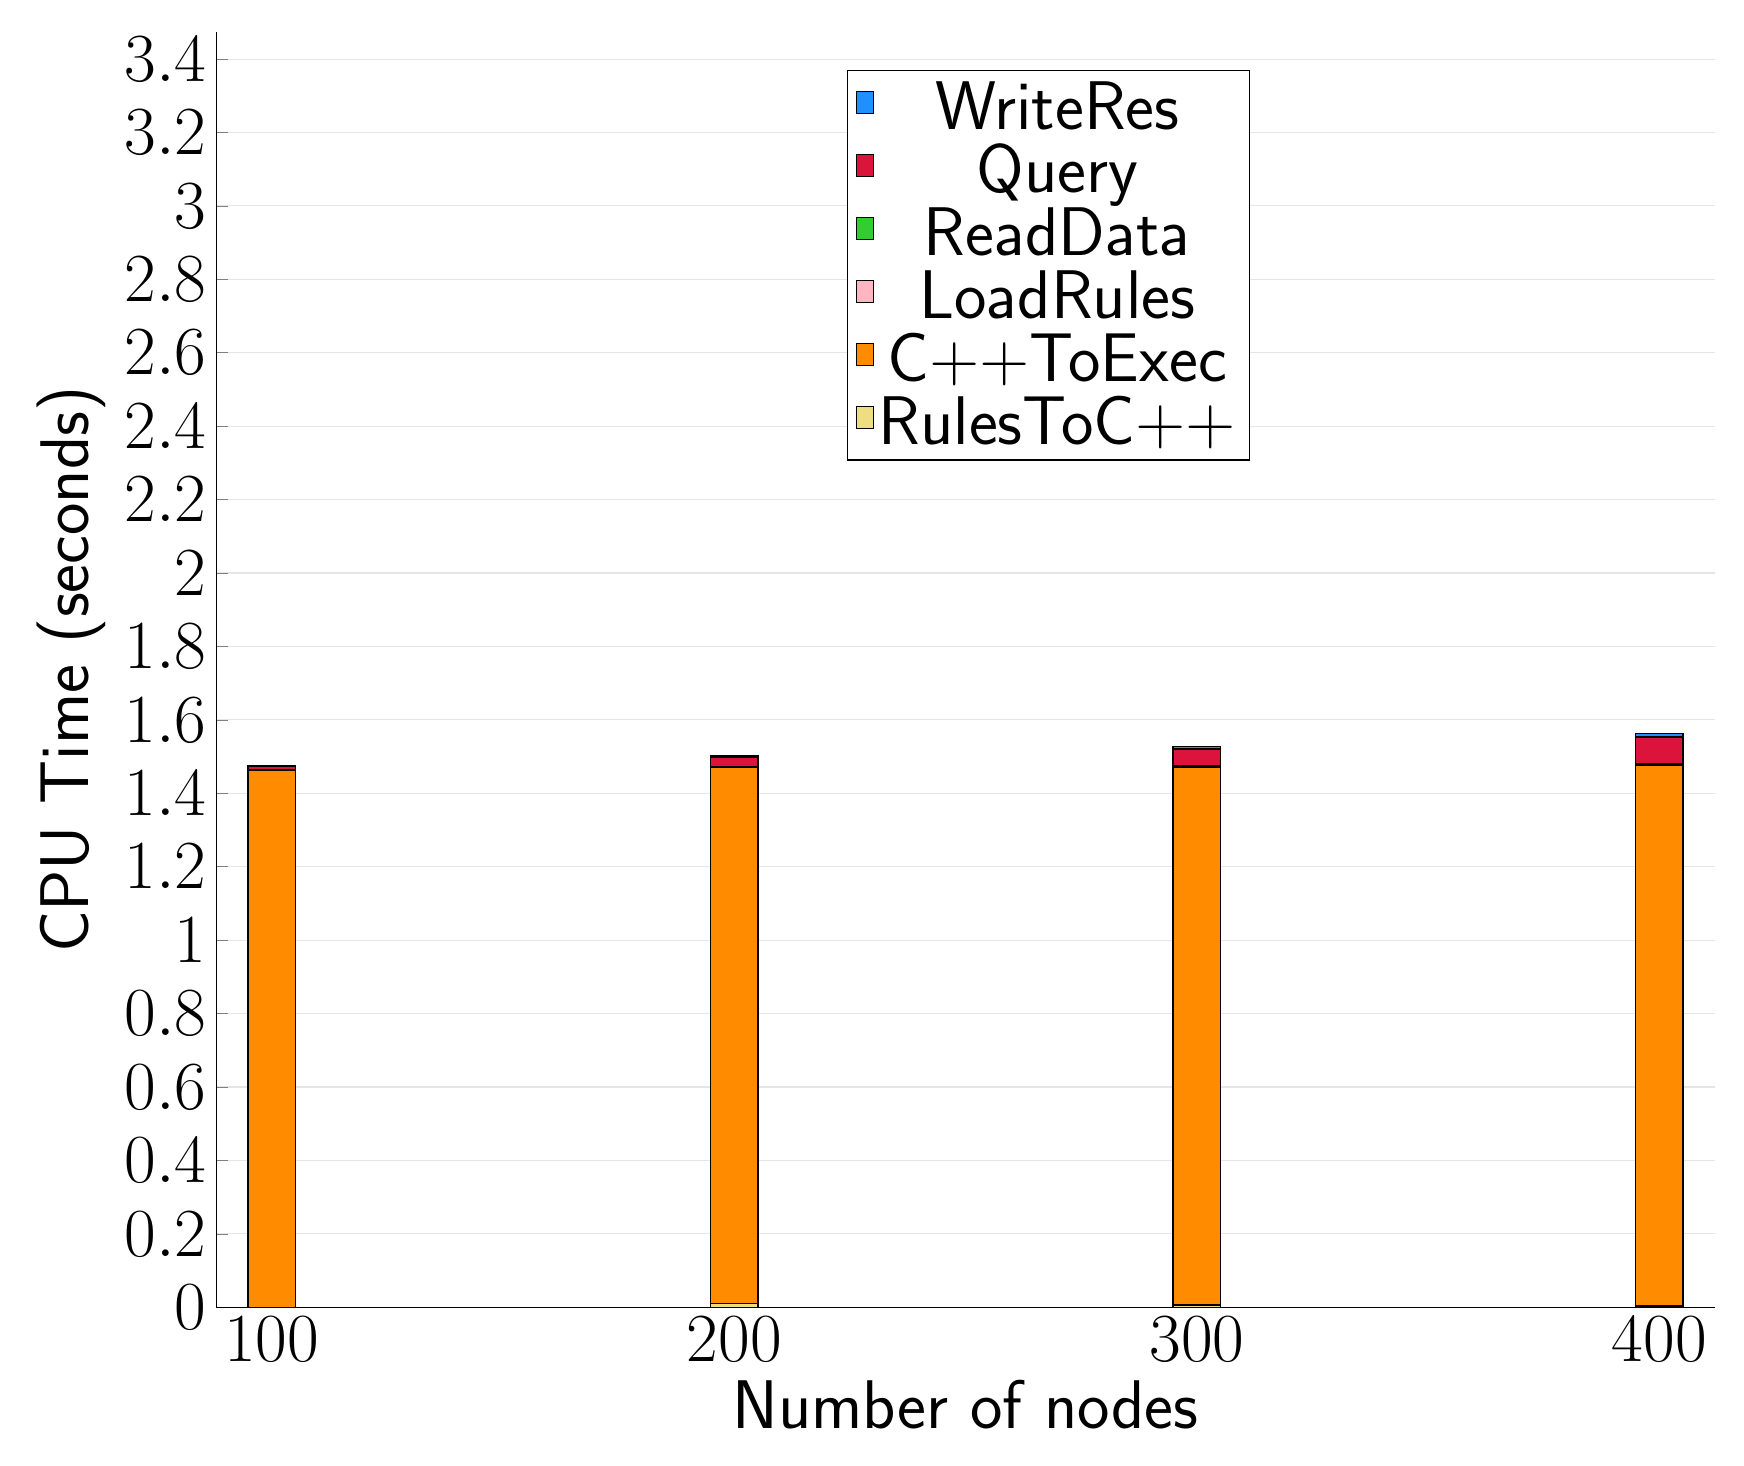
\begin{tikzpicture}
\begin{axis}[
   ybar stacked,
   width=1.7\textwidth,
   bar width=0.6cm,
   ymajorgrids, tick align=inside,
   major grid style={draw=gray!20},
   xtick=data,
   ymin=0, ymax=3.4739999999999998,
   axis x line*=bottom,
   axis y line*=left,
   enlarge x limits=0.04,
   legend style={
       at={(0.69, 0.97)},
       anchor=north east,
       legend columns=1,
       font=\Huge,
   },
   ylabel={CPU Time (seconds)},
   xlabel={Number of nodes},
   label style={font=\Huge},
   tick label style={font=\Huge},
]
\addlegendimage{fill=DodgerBlue, draw=black, line width=0.2pt}
\addlegendentry{WriteRes}
\addlegendimage{fill=Crimson, draw=black, line width=0.2pt}
\addlegendentry{Query}
\addlegendimage{fill=LimeGreen, draw=black, line width=0.2pt}
\addlegendentry{ReadData}
\addlegendimage{fill=LightPink, draw=black, line width=0.2pt}
\addlegendentry{LoadRules}
\addlegendimage{fill=DarkOrange, draw=black, line width=0.2pt}
\addlegendentry{C++ToExec}
\addlegendimage{fill=LightGoldenrod, draw=black, line width=0.2pt}
\addlegendentry{RulesToC++}
\addplot +[fill=LightGoldenrod, draw=black, line width=0.55pt] coordinates {
(100, 0.0)
(200, 0.010000000000000002)
(300, 0.006000000000000001)
(400, 0.004000000000000001)
};
\addplot +[fill=DarkOrange, draw=black, line width=0.55pt] coordinates {
(100, 1.464)
(200, 1.46)
(300, 1.4659999999999997)
(400, 1.472)
};
\addplot +[fill=LightPink, draw=black, line width=0.55pt] coordinates {
(100, 0.0001514)
(200, 0.00015040000000000002)
(300, 0.0001546)
(400, 0.00015780000000000001)
};
\addplot +[fill=LimeGreen, draw=black, line width=0.55pt] coordinates {
(100, 0.0012070000000000002)
(200, 0.0019136000000000001)
(300, 0.00258)
(400, 0.0032714)
};
\addplot +[fill=Crimson, draw=black, line width=0.55pt] coordinates {
(100, 0.0076554)
(200, 0.025887999999999994)
(300, 0.0465858)
(400, 0.0736136)
};
\addplot +[fill=DodgerBlue, draw=black, line width=0.55pt] coordinates {
(100, 0.0016068000000000002)
(200, 0.0039464)
(300, 0.0063592)
(400, 0.0096974)
};
\end{axis}
\end{tikzpicture}

\end{document}
